\chapter{Introduction}
\label{chap:Introduction}

This project focuses on the simulation of a steady-state 3D fluid flow and heat transfer problem within a flow heater, a configuration commonly found in process engineering applications. Accurately predicting both the flow field and temperature distribution is crucial to ensuring a homogeneous process environment, which directly impacts the overall quality of the process.

The geometry of the flow heater is shown in Figure \ref{fig:heater_geo}. For the purposes of this study, a 2D simplification (top-down view) was employed. This reduction in complexity allows for more efficient calculations and comparisons between different turbulence models, while maintaining a reasonable level of accuracy for the task at hand. The study primarily aimed to perform a Grid Convergence Study and evaluate various solver models, with results later applied to custom geometries for further simulations.

The flow heater in this case is examined under both laminar and turbulent flow conditions, leveraging different turbulence models to understand their effect on the heat transfer performance. The comparison of these models plays a key role in identifying the most appropriate solver configuration for real-world applications.

    \begin{figure}[h]   
    \centering
    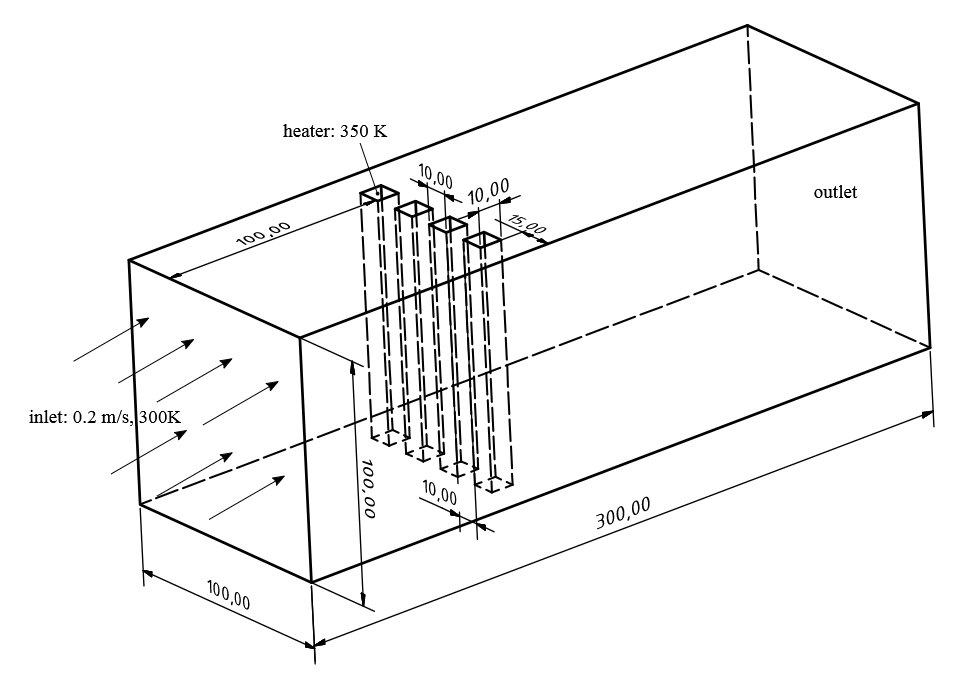
\includegraphics[width=0.65\textwidth]{img/heater_geo_og.png}
    \caption{Given heater geometry}
    \label{fig:heater_geo}
\end{figure}

% EOF
